\documentclass[hyperref={pdfpagelabels=false},unknownkeysallowed]{beamer}
\usepackage{graphicx}
\usepackage{lmodern}
%\usepackage{epstopdf}
%\usepackage[ngerman]{babel}
\usepackage[utf8]{inputenc}
\usepackage{array}
\usetheme{Boadilla}
\usepackage{amsmath}
\usepackage{url}

\setbeamertemplate{note page}[plain]


\def\approxprop{%
  \def\p{%
    \setbox0=\vbox{\hbox{$\propto$}}%
    \ht0=0.6ex \box0 }%
  \def\s{%
    \vbox{\hbox{$\sim$}}%
  }%
  \mathrel{\raisebox{0.7ex}{%
      \mbox{$\underset{\s}{\p}$}%
    }}%
}

%\setbeameroption{show notes}
%\setbeameroption{show only notes}
\setbeameroption{hide notes}

\title{Bayesian Hierarchical Modeling in JAGS}  
\author{Marcel Niklaus} 
\date{\today} 


\begin{document}
	
\begin{frame}
\titlepage
\end{frame} 

\begin{frame}	 
	 \tableofcontents
\end{frame}


\begin{frame}
	\frametitle{Not content of this talk}
	\begin{itemize}
	\item Bayesian Hypothesis test
	\item Model comparison
    \item Too many details
\end{itemize} 
	\note{}
\end{frame}

\section{Why Bayes? What Bayes?}
% % % % % % % % % % % % % % % % % % % % % % % %
\begin{frame}
	\frametitle{Why Bayes: Because it's what you want to know}
	
	\begin{itemize}
	\item We are actually interested in the probability of a model given data
	\item p-values are based on probability of (unobserved) data given model (conceptually hard) 
	\pause
	\item Surprise exercise; think of a situation you are interested in data given model!
	\pause
	\item Bayes rule helps you to get from $p(data|model)$ to $p(model|data)$ 
	\end{itemize} 
	
	\note{In the Bayesian approach we condition on
	the data at hand to assess the plausibility of a hypothesis (via Bayes Rule), while the frequentist approach conditions on a hypothesis to assess the plausibility of the data (or more extreme data sets), with another step of reasoning required to either reject or fail to reject hypotheses.}
\end{frame}


\begin{frame}
	\frametitle{Bayes versus Likelihood approach}
	\begin{itemize}
	\item Maximum likelihood assumption: There is a true fixed value of $\theta$. We maximize the likelihood to estimate it with a certain uncertainty (SE, CI) based on sampling. 
	\item Bayesian way: $\theta$ is a random variable. It has a fixed value, but we reflect our uncertainty about it. 
	\item We summarize the posterior distribution
	\end{itemize} 
\end{frame}


% % % % % % % % % % % % % % % % % % % % % % % %

\begin{frame}
\frametitle{Formal Bayes Theorem}
\begin{center}
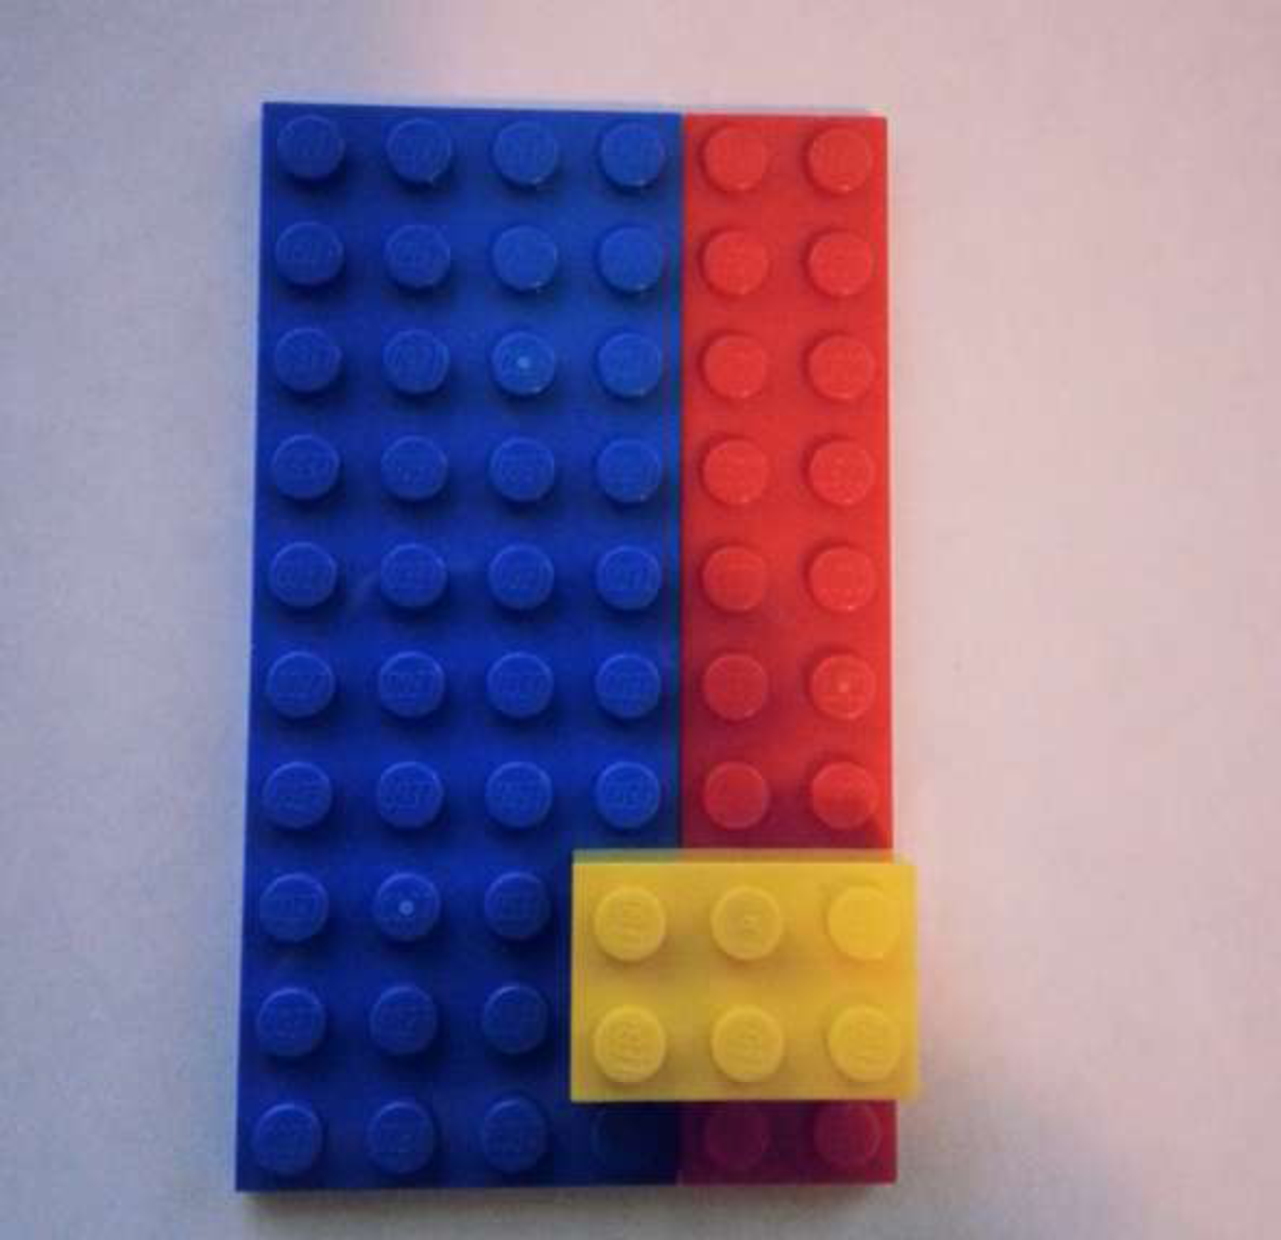
\includegraphics[scale=0.2]{Lego.pdf} 
\end{center}
\begin{itemize}
\item Bayes rule is rooted in conditional probability (and is uncontroversial).
\item $P(Red|Yellow) = P(Yellow|Red) * \frac{P(Red)}{P(Yellow)}$
\item $P(Red|Yellow) = (4/20) * (20/60) / (6/60)$
\item $2 / 3 = 1/5 * 1/3 * 10$
\end{itemize} 
\end{frame}

\begin{frame}
\frametitle{Formal Bayes Theorem (only slide with many formulas)}
\begin{itemize}

\item $P(R|Y) = P(Y|R) * \frac{P(R)}{P(Y)}$
\item Yellow = data, red = hypothesis $\theta$
\item $p(\theta|data)=\frac{p(data|\theta)*p(\theta)}{p(data)}$
\item $posterior = \frac{likelihood * prior}{marginal~likelihood}$
\item $p(\theta|D)\approxprop{p(D|\theta) * p(\theta)}$
\item Posterior is the likelihood weighted by the prior
\item Bayes Theorem tells us how to rationally revise prior beliefs in light of the data to yield posterior beliefs.
\note{ posterior = 2/3, probability of our red model given the yellow data, likelihood is data driven, it's the probability of our yellow data given our red hypothesis, 1/5, times the prior, which is in this case the probability of our red hypothesis = 1/3, divided by the probability of our yellow data, 1/10.}
\note{ marginal likelihood $p(D)$ is only to ensure $\sum = 1$. As a result, this term is often dropped and the Bayes Theorem is written as "proportional to"}
\end{itemize}
\note{ In the frequentist tradition, the assumption is that theta is unknown
but has a fixed value that we wish to estimate. In Bayesian statistical
inference, theta is considered unknown and should be viewed as a random
variable possessing a probability distribution that reflects our uncertainty about the true value of theta.}
\end{frame}


\begin{frame}
\frametitle{General Principles of Bayesian Analysis}
\begin{itemize}
	\item Uncertainty (of parameter estimate) is quantified by probability (distributions)
	\item Observed data is used to update \textbf{prior} information to yield  \textbf{posterior} information
	\item Bayesian workflow: set prior beliefs $\Rightarrow$ get data $\Rightarrow$ update prior beliefs  $\Rightarrow$ summarize posterior beliefs

\end{itemize} 

\begin{center}
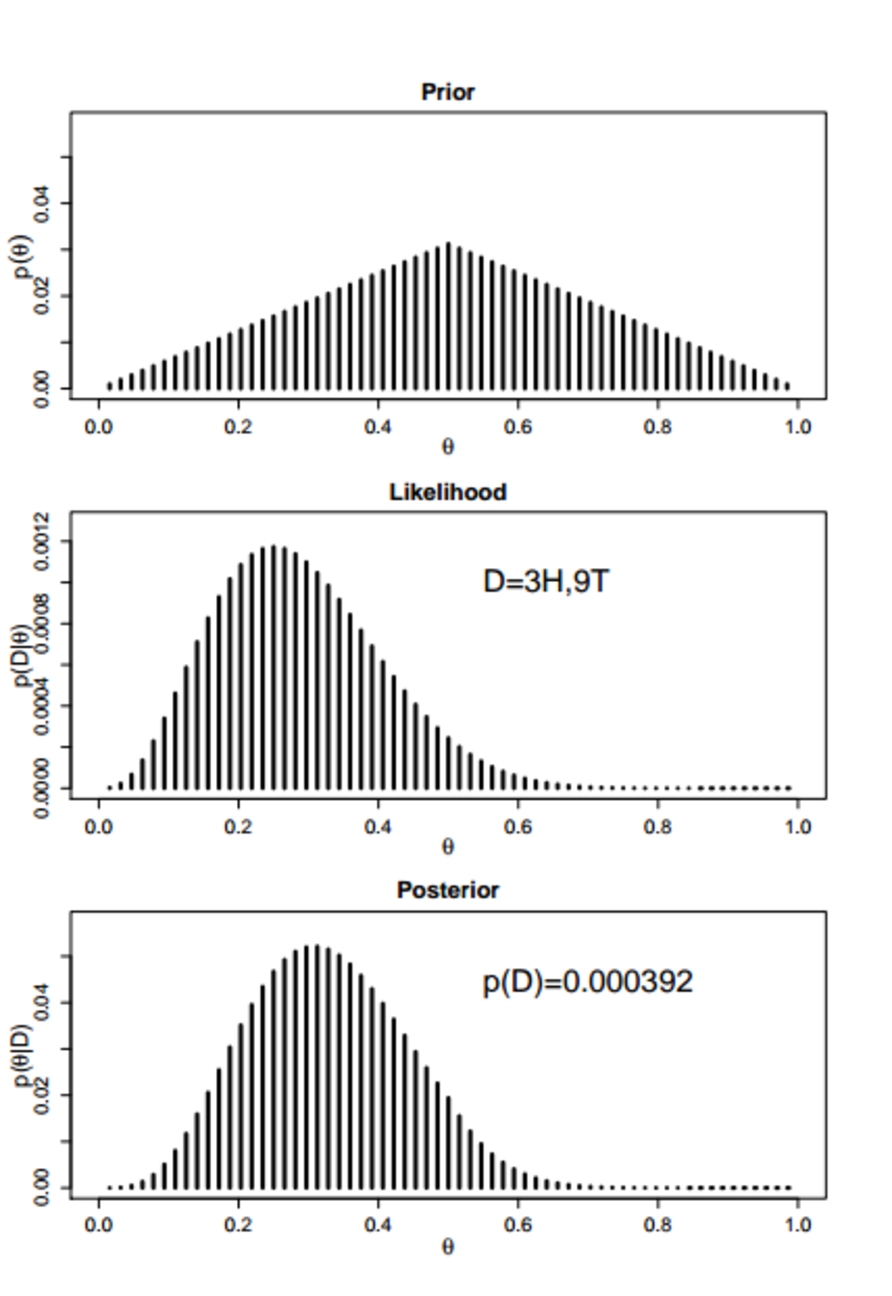
\includegraphics[scale=0.2]{priorlikelihoodposterior.pdf} 
\end{center}
\note{}
\end{frame}

\section{See Bayes: Odd-Even Game}

\begin{frame}
\frametitle{Let's play a game: Odd-Even Guess}

\url{http://87.106.45.173:3838/felix/BayesLessons/BayesianLesson1.Rmd}

\begin{itemize}
\item 6 Trials of Odd-Even Guess )
\end{itemize} 
\end{frame}
% % % % % % % % % % % % % % % % % % % % % % % %

\begin{frame}
\frametitle{Prior}
Pick your Prior: What's your ability? 
\begin{itemize}
\item $\theta$: the rate with which you guess correctly
\item $\theta = 1$: you guess correctly all the time
\item $\theta = 0$: you are terrible at this game
\item $\theta = 0.5$: equal odds
\item Uncertainty (of parameter estimate) is quantified by probability (distributions)
\item We assume our beliefs can be represented by a beta distribution
\item A beta distribution is constraint to lie within 0-1 (perfect for proportion)
\end{itemize}
\note{}
\end{frame}

\begin{frame}
Pick your Prior: What's your ability? 
\begin{itemize}
\item $\theta \sim Beta(1,1)$: Uninformed prior: Do you think (before seeing the data) that it is equally likely that $\theta = 0.01$ and $\theta = 0.5$? 

\item $\theta \sim Beta (3,3)$ : Slightly informed prior
\end{itemize}

We are now ready to play: Go!
\note{}
\end{frame}


\begin{frame}
\frametitle{Likelihood}
The likelihood is the workhorse of Bayesian inference. It represents the data part. 
\begin{itemize}
\item What's the likelihood we observe the data (y wins given n trials)  given the parameter $\theta$ (for each)
\item Probability density of the data, considered as a function of $\theta$
\item The likelihood of a hypothesis conditions on the data as if they are fixed while allowing the hypotheses (our parameter $ \theta$ to vary
\item Binomial likelihood: $L(p|n,y)={n \choose y} p^y (1-p)^{n-y}$

\item \url{http://shiny.stat.calpoly.edu/MLE_Binomial/}
\end{itemize}
\note{}
\end{frame}


\begin{frame} \frametitle{Posterior}
After playing
\begin{itemize}
\item The posterior distribution summarizes our state of uncertainty about the true value of $\theta$ after having observed the game. 
\end{itemize}
\note{}
\end{frame}


\begin{frame}
\frametitle{Markov chain Monte Carlo}
\begin{itemize}
\item Posterior distribution = Prior distribution $*$ Likelihood density
\item Analytical calculation of posterior only possible for simple models (high-dimensionality integration problem)
\item Draw samples from posterior and summarize the distribution of those samples (it works!)
\item MCMC: algorithm that whose draws are dependent on previous draw. This chain will converge to the posterior.  
\item Metropolis-Hastings algorithm and the Gibbs sampler (google it!)
\item JAGS WinBugs and STAN can do this for you
\item Algorithm to approximate an unknown distribution

\end{itemize}
\note{Specifically, at each iteration, the algorithm picks a candidate for the next sample value based on the current sample value. Then, with some probability, the candidate is either accepted (in which case the candidate value is used in the next iteration) or rejected (in which case the candidate value is discarded, and current value is reused in the next iteration)−the probability of acceptance is determined by comparing the values of the function f(x) of the current and candidate sample values with respect to the desired distribution P(x).}
\end{frame}



% % % % % % % % % % % % % % % % % % % % % % % %
\section{Easy Example in JAGS}

\begin{frame}
	\frametitle{JAGS Basics}
	\begin{itemize}
	    \item $\leftarrow$ is~equal~to: $y \leftarrow a+b$
	    \item $\sim$ is distributed as..
	    \item Binomial likelihood: $y \sim dbin(\theta,nAttempts)$
		\item Normal likelihood: $ y \sim dnorm(mean,precision)$
		\item $precision = 1/ Var$
		\item Loop: for (i in 1:3)\{bla[i]=1+i\}
		\item bla = 2,3,4, bla[2] = 3
		\item order of commands is irrelevant
	\end{itemize} 
	\note{}
\end{frame}

\begin{frame}
\frametitle{Soccer Shootout}
Let's estimate soccer players' ability to score a penalty in a world cup! 
\begin{itemize}
\item Open Soccer.R in your R console
\item Set your working directory (line 8)
\item Jags model: ShootoutAbility.txt
\item What is their ability $\theta$, [0-1]?
\item $Y\theta$ Prior: remember the game
\item Credible interval: $\theta$ lies between lower and upper bound  with a probability of 95\%. 
\end{itemize}
\note{}
\end{frame}


\begin{frame}
Convergence: Has the MCMC Gibbs sampler converged on posterior (after starting from random values)
\begin{itemize}
\item Trace plot: "fat, hairy caterpillar"
\item Autocorrelation plot: "Chains should forget previous visits with time": drop off quickly: thinning
\item Gelman-Rubin-Brooks diagnostic: Between and within chain variance: 1 indicates convergence (F-value); less than 1.2. See gelman.diag [CODA]
\item Geweke test of non-stationarity; Heidelberger-Welch test etc.
\end{itemize}
\note{}
\end{frame}

\begin{frame}
\frametitle{Soccer Shootout: Afrika vs. Europa and America}
\begin{itemize}
\item Jags model: ShootoutAbilityDifference.txt
\item theta[Cindex[i]] can either be theta[1], or theta[2]
\item estimates separate parameters for Africa and Europe \& America
\end{itemize}
\note{}
\end{frame}


\begin{frame}
\frametitle{Critiques}
Bayesians use unjustified priors
\begin{itemize} \item Frequentists use uninformative priors \end{itemize}
Subjective priors dominate the results
\begin{itemize} \item data overwhelm the prior with enough n \end{itemize}
And also...
\begin{itemize} \item Bayes factors are consistent: With large N, Bayes statistics will tell you if null hypothesis is true \end{itemize}
\note{}
\end{frame}


%%%%%%%%%%%%%%%%%%%%%%%%%%%%%%%%%%%%%%%%%%%%%%%%%%%%%%%%%%%%%%%%%%%%%%%%%%%%
%%%%%%%%%%%%%%%%%%%%%%%%%%%%%%%%%%%%%%%%%%%%%%%%%%%%%%%%%%%%%%%%%%%%%%%%%%%%

\section{Hierarchical Modeling}
\begin{frame}
\frametitle{Hierarchical Modeling}

\begin{itemize}
\item With nested data (e.g. data for participants is organized on more than 1 level), a multilevel model is appropriate. 

\item The classic: students grouped in classes, which nest in school districts, which in turn nest in states. 


\item Many names: Mixed effects modeling, multi-level modeling... Bayesian hierarchical modeling gets rid of these confusions. 
\item All Bayesian Models are hierarchical because every parameter has a prior. 
\item All parameters in bayesian models are random effects
\end{itemize} 

\note{}
\end{frame}

% % % % % % % % % % % % % % % % % % % % % % % %

\begin{frame}
\frametitle{Easy IQ example: IQ measurements}
Ignore the grouping variable: 1 $\mu$ for all:
\begin{itemize}
    \item Scenario: We measure some IQs
	\item $y \sim N(\mu,\tau)$
    \item $\mu \sim N(100,0.004)$ 
    \item $\tau \sim Gamma(0.001,0.001)$
    \end{itemize} 
\note{}
\end{frame}


\begin{frame}
\frametitle{Intercept varies by group}
\begin{itemize}
    \item Scenario: We measure some IQs
	\item $y \sim N(\mu[G],\tau)$
    \item for each Group G :$\mu[G] \sim N(100,0.004)$ 
    \item $\tau \sim Gamma(0.001,0.001)$
    \item This estimates G means
    \end{itemize} 
\note{}
\end{frame}

\begin{frame}
\frametitle{Hierarchical Model}
\begin{itemize}
    \item Instead of assuming a completely different mean for each Group G, we assume that they are drawn from a common Normal distribution
    \item "Random" means we draw the values from a normal distribution 
\item $y \sim N(\mu[G],\tau)$ 
\item for each Group G:  $\mu[G] \sim N(Hypermean,HyperSD)$
\item $Hypermean \sim N(100,0.0044)$
\item $HyperSD \sim Gamma(0.001,0.001)$
    \end{itemize} 
\note{}
\end{frame}


\begin{frame}
\frametitle{Linear Mixed Models}

\begin{itemize}
\item Linear Regression model
\item Mixed because it includes coefficients that vary over group (random: participants, items) and some that don't (fixed, treatment group). 
\item Random Effects: zero mean restriction $N(0,\omega)$)
\item Random intercepts model: random intercept, fixed slope
\item Random intercepts and slope model: random intercept, random slope
\end{itemize} 
\centering In Bayesian Statistics, all parameters are random, i.e. drawn from an overarching distribution!  
\note{}
\end{frame}


\begin{frame}
\frametitle{Fixed Effects Model: Math grade and IQ}
Ignore the grouping variable
\begin{itemize}
\item $y \sim N(\mu,\tau)$
\item $\mu <- ~~x0 + x1 * math$
\end{itemize} 
\note{}
\end{frame}

\begin{frame}
\frametitle{Random Intercept}
\begin{itemize}
\item $y \sim N(\mu,\tau)$
\item $\mu <- x0[G] + x1 * math$
\item for all groups j: $x0[j] \sim N(hypermean,hypersd)$
\item $hypermean \sim N(100,0.004)$
\item $hypersd \sim Gamma(0.001,0.001)$
\item $x1 \sim N(0,0.001)$
\end{itemize} 
\note{}
\end{frame}

\begin{frame}
\frametitle{Random Intercept: 2}
\begin{itemize}
\item $y \sim N(\mu,\tau)$
\item $\mu <- x0+ u0[G] + x1 * math$
\item for all groups g: $u0[g] \sim N(0,hypersd)$
\item $x0 \sim Uniform(-\infty,\infty)$
\item $x1 \sim Uniform(-\infty,\infty)$
\item $hypersd \sim Uniform(-\infty,\infty)$
\end{itemize} 
\note{}
\end{frame}



\begin{frame}
\frametitle{Random Intercept and Slope}
\begin{itemize}
\item $y \sim N(\mu,\tau)$
\item $mu <- x0[G] + x1[G] * math$
\item for all groups g: $x0[g] \sim N(hypermeanintercept,hypersdint)$
\item for all groups g: $x1[g] \sim N(hypermeanslope,hypersdslope)$
\item $hypermeanintercept \sim N(100,0.004)$
\item $hypermeanslope \sim N(0,0.001)$
\item $hypersdint \sim Gamma(0.001,0.001)$
\item $hypersdslope \sim Gamma(0.001,0.001)$
\end{itemize} 
\note{}
\end{frame}


\begin{frame}
\frametitle{Variance-Covariance Matrix}
\begin{itemize}
\item if random slopes and random intercepts may not be independent
\item Google cholesky decomposition! 
\end{itemize} 
\note{}
\end{frame}

\begin{frame}
\frametitle{Multi-level Models}
\begin{itemize}
\item $y \sim N(\mu,\tau)$
 \item $\mu \sim N(\mu2,\tau2)$
 \item $\mu2 = z0+z1*level2covariate$ 
 \item random intercept and slopes can be given if there are even more levels
  \item $\mu2 = z0[level2Groups]+z1*level2covariate$ 
 \end{itemize} 
\note{}
\end{frame}


\section{Linear Mixed Effects model in JAGS}

\begin{frame}
\frametitle{Simple linear regression}
London school match-exam tests and London Reading Test scores 
\begin{itemize}
\item Open Exam${\_}$ple.R in your R console
\item Set your working directory (line 7)
\item Jags model: ExamSimple.txt
\end{itemize}
\note{}
\end{frame}

\begin{frame}
\frametitle{Random intercept model}
\begin{itemize}
\item b0[school[i]]
\item for all schools: $b0[j] \sim dnorm(school.b0,school.tau) $
\item $school.b0 \sim dnorm(0,0.0001)$
\item all j school means are drawn from school.b0
\end{itemize}

\note{}
\end{frame}

\begin{frame}
\frametitle{Random intercept and slope model}
\begin{itemize}
\item $b0[school[i]]+b1[school[i]]*lrt[i]$
\item for all schools: $b0[j] \sim dnorm(school.b0,school.tau) $
\item for all schools: $b1[j] \sim dnorm(school.b1,school.tau.b1)$
\item school.b0 $\sim$ dnorm(0,0.0001)
\item school.b1 $\sim$ dnorm(0,0.0001)
\item all j intercepts and slopes are drawn from a Normal with estimated hyperparameters
\end{itemize}
\note{}
\end{frame}

\section{Multilevel Model}

\begin{frame}
\frametitle{Multi-Level Models}
Covariates that capture the way groups vary are included

\begin{itemize}
\item Level 1: Regression for London Reading Test
\item Level 2: Group Level with covariates: Regression for entry score
\item b0[j] $\sim$ c0+c1$*$ entry[j]
\end{itemize}
\note{}
\end{frame}

% % % % % % % % % % % % % % % % % % % % % % % %
\begin{frame}
\frametitle{Multi-Level Models}
Covariates that capture the way groups vary are included

\begin{itemize}
\item c0: intercept
\item c1: effect of entry (L2) on intercept
\item d0: effect of LRT 
\item d1: effect of entry on LRT effect
\end{itemize} 
\note{}
\end{frame}

% % % % % % % % % % % % % % % % % % % % % % % %
\end{document}
